\documentclass[12pt]{article}

\usepackage{sbc-template, placeins}
\usepackage{graphicx,url, subfigure, multirow, comment}
\usepackage[utf8]{inputenc}
\usepackage[brazil]{babel}
%adicionados manualmente
\usepackage{tabularx}
\usepackage{multirow}  

     
\sloppy

\title{Digite o Título aqui}

\author{Seu Nome Completo aqui, Nome completo do orientador aqui}

\address{Coordenação do Tecnólogo em Análise e Desenvolvimento de Sistemas (ADS) \\ Instituto Federal do Piauí (IFPI) - Campus Pedro II \\
  Rua Antonino Martins de Andrade, 750 -- 64.255-000 -- Pedro II -- PI -- Brazil
\email{\{aluno\}@aluno.ifpi.edu.br, idorientador@ifpi.edu.br}
}

\begin{document} 

\maketitle

\begin{abstract}
  This meta-paper describes the style to be used in articles and short papers
  for SBC conferences. Abstracts should not have more than
  10 lines and must be in the first page of the paper.
\end{abstract}
     
\begin{resumo} 
  Fazer este item por último. É solicitada a escrita de resumo e abstract apenas para os artigos escritos em português. Artigos em inglês deverão apresentar apenas abstract.
  Nos dois casos, o autor deve tomar cuidado para que o resumo (e o abstract)
  não ultrapassem 10 linhas cada, sendo que ambos devem estar na primeira
  página do artigo.
\end{resumo}


\section{Introdução}

Aqui deverá ser escrita a introdução do seu artigo, não esqueça de seguir a notas de aula para compor um contexto forte e embasado na literatura. Siga os modelos de aula e não esqueça de retirar as dúvidas com o professor da disciplina.

Edite o texto como preferir e siga os itens específicos do template. Lembre que você pode adicionar pacotes no preâmbulo e customizar o conteúdo das seções.

\section{Referencial Teórico} \label{sec:ref-teorico}

Esta seção apresenta o referencial teórico ou revisão de literatura. Utilize o modelo para inserir seu texto com seções pertinentes a cada item relevante para sua escrita.

Não esqueça de citar e abordar trabalhos diretamente relacionados reforçando sua jutificativa nos parágrafos finais.

\section{Metodologia}

Esta seção apresenta a metodologia ou materiais e métodos empregados para realização do projeto. É o cerne de seu projeto onde voce indica exatamente o \textbf{como fazer}. 

É importante nos parágrafos finais dar enfase aos possíveis resultados esperados ja que em projetos de pesquisa não se usa uma seção de  resultados.

\subsection{Sub seção XX}

Lembre de adicionar subsessões sempre que achar necessário para melhorar o fluxo da leitura.

\section{Exemplos de Figuras and Captions}


Esta seção apresenta exemplos de  figuras e outro itens no formato SBC que podem ser usados como modelos em outras seções. Recomenda-se deixar esta seção para usar como modelo e posteriormente excluí-la por completo. Seguem exemplos de figura, tabelas e outros itens úteis. Lembre-se que as citações no seu arquivo de referências aparecerão no texto a medida que usar o comando cite.

\begin{figure}[ht]
\centering
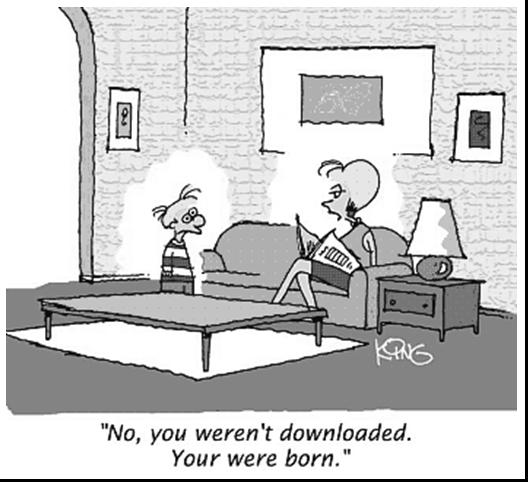
\includegraphics[width=.5\textwidth]{fig1.jpg}
\caption{A typical figure}
\label{fig-identificador-figura}
\end{figure}

Em tabelas, o caption deve ser localizado antes  das tabelas (see Table 1)
e a fonte deve ser Helvetica, tamanho 10, com 6 pontos de espaço antes e depois de cada caption.

\begin{table}[ht]\footnotesize
\centering
\caption{Titulo de sua tabela}
\begin{tabular}{l r r r}
\hline
Nome & Prova 1 & Prova 2 & Média\\
\hline
João Silva & 5{,}0 & 6{,}0 & 5{,}5\\
Maria Oliveira & 7{,}0 & 6{,}0 & 6{,}5\\
Isabela Medeiros & 8{,}6 & 9{,}4 & 9{,}0\\
\hline
\end{tabular}
\label{tab:csvdescription}
\end{table}

O exemplo de  tabelapod ser alterado para usar o ambiente tabularx e criar tabelas com linhas e colunas mais flexíveis. Pode-se usar  tabelas simples seguindo as recomendações do template para manter a formatação.

%comandos que inserem a bibliografia contida no arquivo referencias.bib
\bibliographystyle{sbc}
\bibliography{referencias}

\end{document}
